\section{PS2: Sokoban}\label{sec:ps2}

\subsection{Overview}\label{sec:ps2:overview} % A discussion of the assignment itself

In this assignment, we were tasked with making a simple version of the game Sokoban which is a simple 2d block-pushing game.
The program was to be run with a given level file that contained a grid of characters representing the starting game state.
The game includes the ability of being able to move the player around using WASD and reset the level using 'R'. 
The boxes/storage containers are able to be pushed around the game area with the goal of putting them into the storage spaces.
Once all the boxes are in the storage spaces or all storage spaces are filled with boxes thed the game is won.

\subsection{End Product}\label{sec:ps2:accomplish} % What I accomplished and images/results

Below is the output.
Level one is being played.
On the left is the starting game state.
On the right is the game being won.

\begin{figure}[h]
\centering
\begin{minipage}[b]{0.4\textwidth}
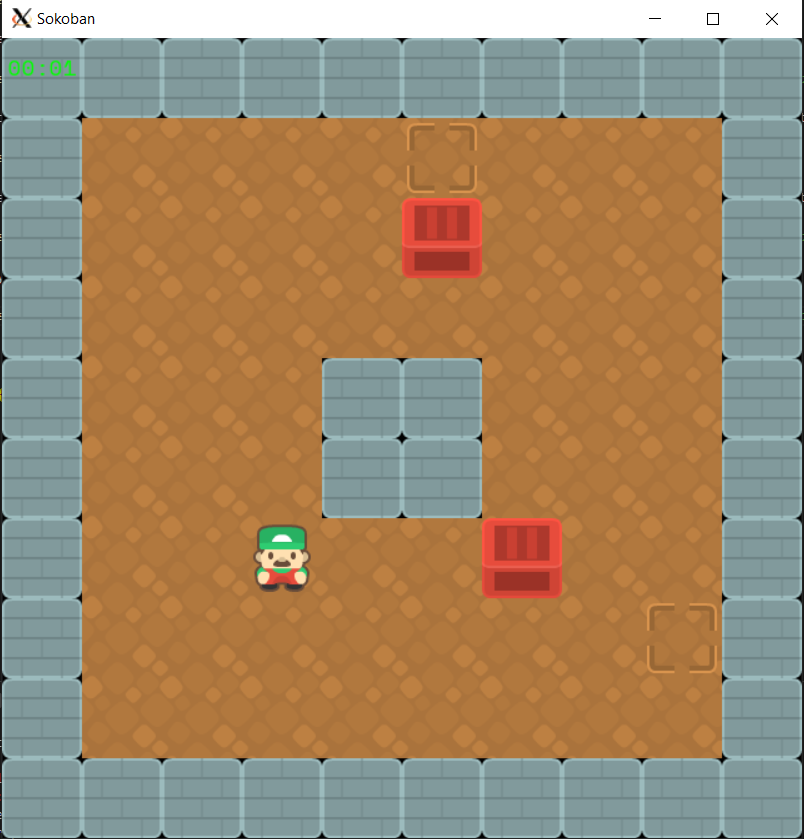
\includegraphics[width=\textwidth]{ps2-1_output}
\caption{Level 1 Start}
\end{minipage}
\hfill
\begin{minipage}[b]{0.4\textwidth}
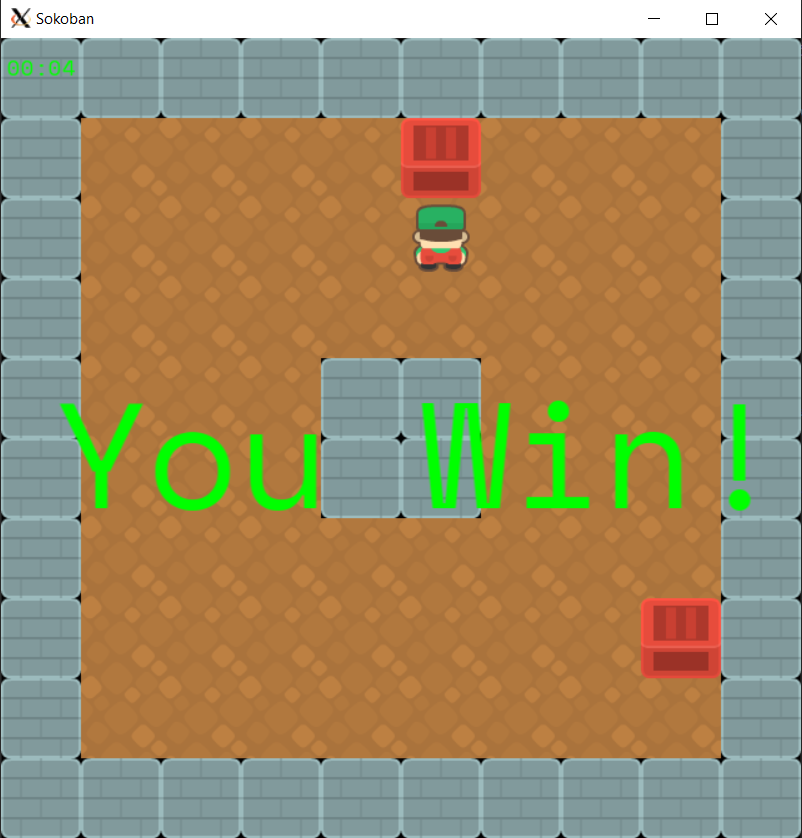
\includegraphics[width=\textwidth]{ps2-2_output}
\caption{Level 1 Won}
\end{minipage}
\end{figure}

\subsection{What I Already Knew}\label{sec:ps2:knew} % What was known prior to the assignment

I knew some basics of SFML for sprite movement and drawing to the screen.
As for C++, I knew a variety of containers that could be used to develop the class.
I also had past experience of implementing game mechanics/boundary conditions from previous school and personal projects.

\subsection{Design Decisions and Implementations}\label{sec:ps2:decisions} % Important decisions or implementations I made

For the game internals  I created a Sokoban class. To display the game, I separated the game field into many different object containers.
I first made a vector of textures that were loaded in once. 
These were to be shared between multiple sprites because sprites take up far less memory than textures, so this improved load speeds and reduced memory usage.
I then made a 2d vector of characters to hold an exact copy of level file. This was for ease of access later on for game mechanics. 
As for displaying the game, I separated the environment(walls and floors), storage containers/boxes, storage spots, and the player into different sprite containers.
This made it so that certain game elements could be drawn over each other/have same positions, such as the player standing on the floor. 
To display these, the class inherited from SFML draw class and the 'draw' function was overloaded so if you called 'draw' with a Sokoban object it would draw the whole game out.

\bigskip
As for the core game mechanics, I controlled most of them through the 'movePlayer' and 'isWon' functions.
In the 'movePlayer' function I made a vector of x,y pairs that represented the displacement after a key press.
This made it so I could generalize the game mechanics across keystroke presses to reduce the code four fold.
For each movement I checked that it wouldn't be an illegal movement and would act appropriately with the box.
For the player, that meant they could not go out of bounds, through a wall, or into a box.
However, the player should be allowed to push a box, unless another box was in front of it, or by pushing the box it would go out of bounds or through a wall.
If any such illegal movement was attempted, the 'movePlayer' made sure no such movement was made.
If there were no illegal actions being made the respective sprite's positions were updated.

\bigskip
In the isWon function there was a few scenarios where the player would win.
If there were equal boxes to spaces, or more boxes than spaces, the player won once all the storage spaces were filled. 
If there were more spaces than boxes, the player won once all the boxes were in a storage location.
To account for all of them the lower number between the number of boxes and the number of storage spaces could be used to determine when the game was won.
To check if boxes were in storage spaces I looped through the vectors of both. For each box/storage combination I compared their position using the 'find\_if' algorithm paired with a lambda function. 
If by the end of looping the number of boxes in storage spots met that determined lower number, then the player had won. 

\bigskip
For extra credit, I added a few different things.
I first added a timer in the top left that counted the time passed after the level began.
Some small features I added were a victory sound when the game was won, and a player model change when the player's direction changed.
As a custom feature I added the ability for the player to play the next level if 'N' is pressed or play the previous level if 'P' is pressed after completing current level.
To go to the next/previous level that level must exist or the game will just remain on the winning screen.

\subsection{What I Learned}\label{sec:ps2:learned} % What I learned because of the assignment

I continued learn more about SFML, especially sprites and their possible functions.
I learned how to properly overload the draw function for user made classes/objects.
I learned/used lambda functions for the first time.

\subsection{Challenges}\label{sec:ps2:challenges} % Challenges along the way and any that went unresolved

Everything turned out how I wanted it, but this was the first project with some more challenging problems.
The first big trouble I had was overloading the draw function;
it was simple after I completed it, but it was hard to find how to overload it properly using SFML API, so it became somewhat of a trial and error.
In general it was tough to figure out how I wanted my game to be represented, so I was constantly making more containers to hold the game objects.
In the gameplay part of the project, just eliminating all of the possible boundary conditions for movement took a little while.
The hardest challenge was trying to center the victory text, but  that too felt like was because of SFML API.

\newpage
\subsection{Codebase}\label{sec:ps2:code} % Code: Makefile, .cpp main, .hpp main, .cpp support, .hpp support, .cpp tests

\bigskip
\title{\large Makefile:}
\lstinputlisting{../ps2b/Makefile}
\bigskip
\title{\large main.cpp:}
\lstinputlisting{../ps2b/main.cpp}
\bigskip
\title{\large Sokoban.cpp:}
\lstinputlisting{../ps2b/Sokoban.cpp}
\bigskip
\title{\large Sokoban.hpp:}
\lstinputlisting{../ps2b/Sokoban.hpp}

\newpage
